The following sections are dedicated to the Wireless Communications Layer of this project. This layer includes the Ethernet Subsystem and the Black Box Subsystem. The Wireless Communications Layer manages the communications demands between the Web Interface Layer and the Camera Layer via UDP transport protocol over a wireless network provided the consumer by TrafficNet LLC.

\subsection{Wireless Communications Layer}
User issued commands will be sent from the Web Interface Layer to the Black Box Subsystem via UDP/IP Transfer Protocol, and subsequently forwarded by the Ethernet Subsystem to the Raspberry Pi Zero for execution.   

\subsection{Wireless Communications Layer Hardware}
Specifically, the Wireless Communications Layer is comprised of a TBD Wireless Network Adapter of TrafficNet, LLC's choosing and the Ethernet Adapter connected to the Raspberry Pi Zero. The two components work in tandem to provide a means through which the Raspberry Pi Zero can establish communication with the Web Interface Layer.

\subsection{Layer Software Dependencies}
It is necessary for the appropriate software to be present on the Raspberry Pi Zero to provide the end connection for the video streaming server to operate through. This software runs the UDP/IP Transfer Protocol which allows the video to be streamed wirelessly to the Web Interface Layer. It is the TrafficNet.py program described in the Camera Layer.

\subsection{Black Box Subsystem}
The Black Box is a placeholder name for the indeterminate Wireless Network Adapter to be incorporated by the vendor TrafficNet, LLC at a later date. However, it is crucial to the operation of the Wireless Communications Layer. Regardless of the specifics of the chosen WNA, its function will remain the same. Without it there can be no connection established between the ports of the user's machine and the Raspberry Pi Zero.

\begin{figure}[h!]
	\centering
 	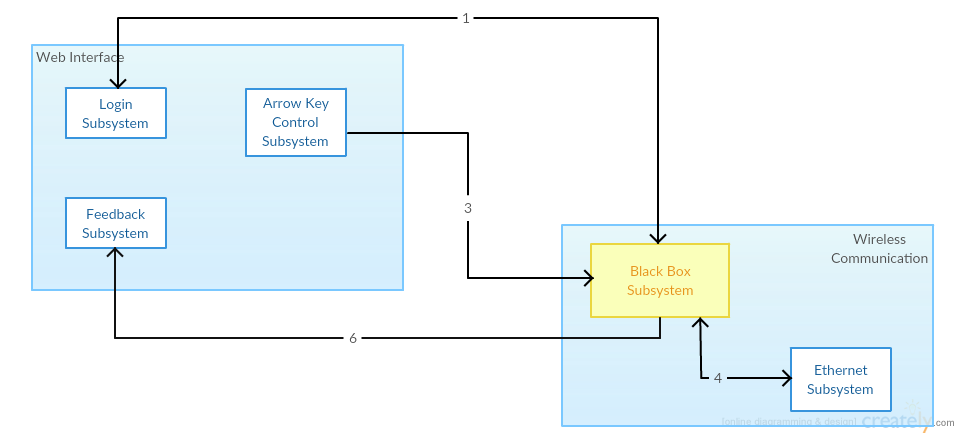
\includegraphics[width=0.60\textwidth]{architectural design specification latex/images/ADSdiagrams/blackboxsubsystem.png}
 \caption{Black Box Subsystem description diagram}
\end{figure}

\subsubsection{Black Box Subsystem Hardware}
The specific WNA at this time is unknown.

\subsection{Ethernet Subsystem}
The Raspberry Pi Zero has an Ethernet Adapter connected to it. This is Ethernet Subsystem of the Wireless Communications Layer. It connects the Raspberry Pi Zero to the WNA of the Black Box Subsystem.

\begin{figure}[h!] 
 	\centering 
  	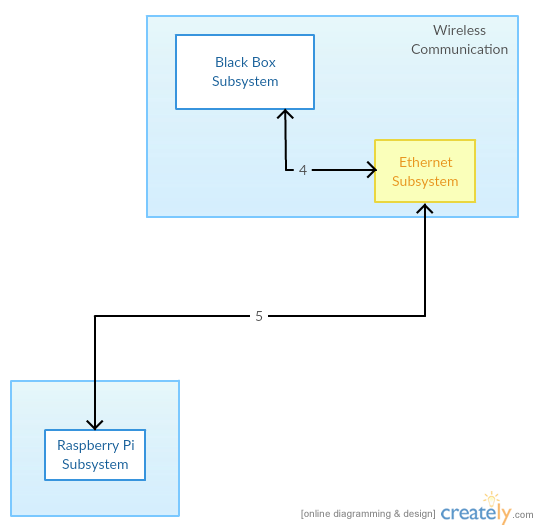
\includegraphics[width=0.60\textwidth]{architectural design specification latex/images/ADSdiagrams/ethernetsubsystem.png} 
 \caption{Database Subsystem Description} 
\end{figure}

\subsection{Ethernet Subsystem Hardware}
The Ethernet Adapater is a Micro-USB 2.0 to Ethernet Port OTG Cable capable of communication speeds up to 100Mbps.

\subsection{Ethernet Subsystem Software Dependencies}
The Ethernet Adapter comes with pre-installed drivers for 802.3 Network Standards.
